\section{Large Scale Linear Algebra and Optimization for Data-Intensive Calculations}

\subsection{Laplace Interpolation} \label{ss:laplace}
The punch-and-fill algorithm is the most expensive computational step in computing the 3D-$\Delta$PDF in the standard workflow. The punch-and-fill algorithm involves the removal of Bragg peaks and ``fills" the data in the region of the Bragg peaks. Previously, the Bragg peaks were filtered by convolving with Gaussian smoothing operator. The Gaussian Smoothing Operator performs a weighted average of surrounding pixels based on the Gaussian distribution. While this approach filtered Bragg peaks well, it is computationally expensive ($\mathcal{O}(n^3 \log(k))$, where $n\times n \times n $ is the size of the volume data and the size of the Gaussian kernel is $k \times k \times k$). The smoothing using Gaussian Kernels has to performed using the entire dataset and does not easily lend itself for parallelization. 

To overcome this computational limitation, we developed a linear interpolation technique such that the missing data satisfies the 3-D Laplace difference equations. This has the following advantages: a) it results in a banded linear system of equations (tridiagonal for 1D, pentadiagonal for 2D and so on) sparse and hence one can leverage many sparse linear algebra techniques and software packages, b) another major advantage is instead of solving a single large linear system, one can solve smaller local linear systems corresponding to each Bragg peak and this operation is embarrassingly parallel. For example for a 3D volume data with 125M pixels (500 $\times$ 500 $\times$ 500) -- instead of solving a large 125M by 125M linear system, one can solve 1000 10K by 10K linear systems in parallel. This results in great computational savings (for the 3D VO$_2$ data, we observed a six- to ten-fold reduction in compute time. This can be further enhanced by using parallel computing resources). Figure \ref{fig:punch_and_fill} shows a 1-D slice of the results of punch and fill using the Laplace interpolation on the VO$_2$ dataset. One notes that the performance of the new method is broadly comparable to the old one, but it is \textit{much faster}. The Laplace interpolation and a generalization of the Laplace interpolation -- called the Matern interpolation has been published as a Julia package (\texttt{LaplaceInterpolation.jl}) and more details about the package can be found in our paper \cite{RH2022}.

\begin{figure}
     \centering
     \begin{subfigure}[b]{0.45\textwidth}
         \centering
         \includegraphics[width=\textwidth]{Figures/BraggPeaks.png}
         \caption{1-D slice with Bragg Peaks}
         \label{fig:BraggPeaks}
     \end{subfigure}
     \hfill
     \begin{subfigure}[b]{0.45\textwidth}
         \centering
         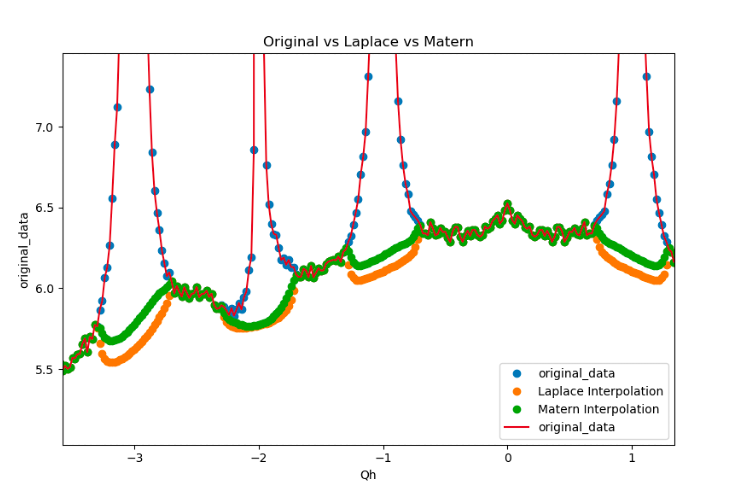
\includegraphics[width=\textwidth]{Figures/Punch_Fill.png}
         \caption{1-D slice after punch-and-fill}
         \label{fig:punch_fill}
     \end{subfigure}
        \caption{1-D slice with punch-and-fill using both Laplace and Matern Interpolation}
        \label{fig:punch_and_fill}
\end{figure}
% \begin{figure}
% 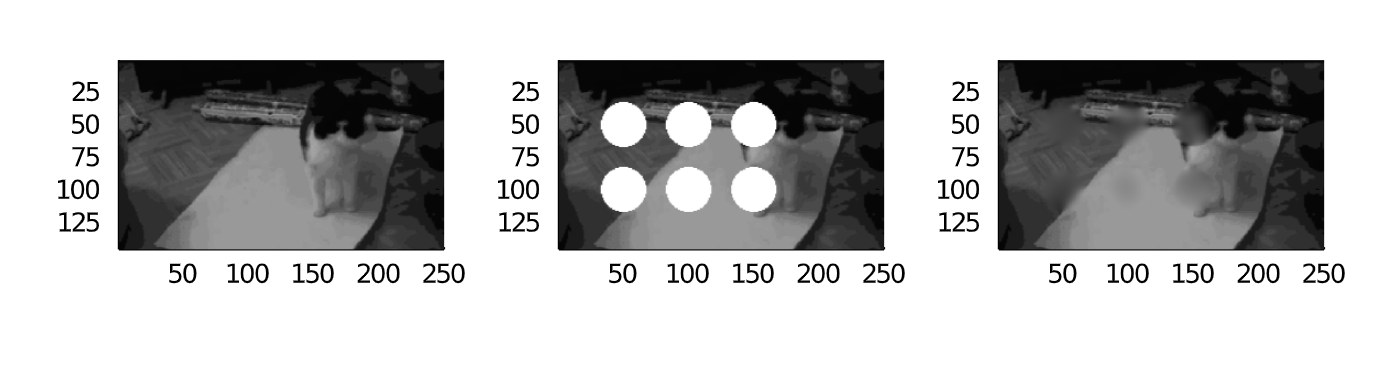
\includegraphics[width=\textwidth, trim=0in 4in 0in 4in 0in]{Figures/LaplaceInterp_3D.png}
% \caption{\label{fig:punch_and_fill} Left panel shows the original data, the center panel shows the right panel shows the data after punch and right frame shows the data after fill}
% \end{figure}
\subsection{Compressed sensing}

\begin{figure}
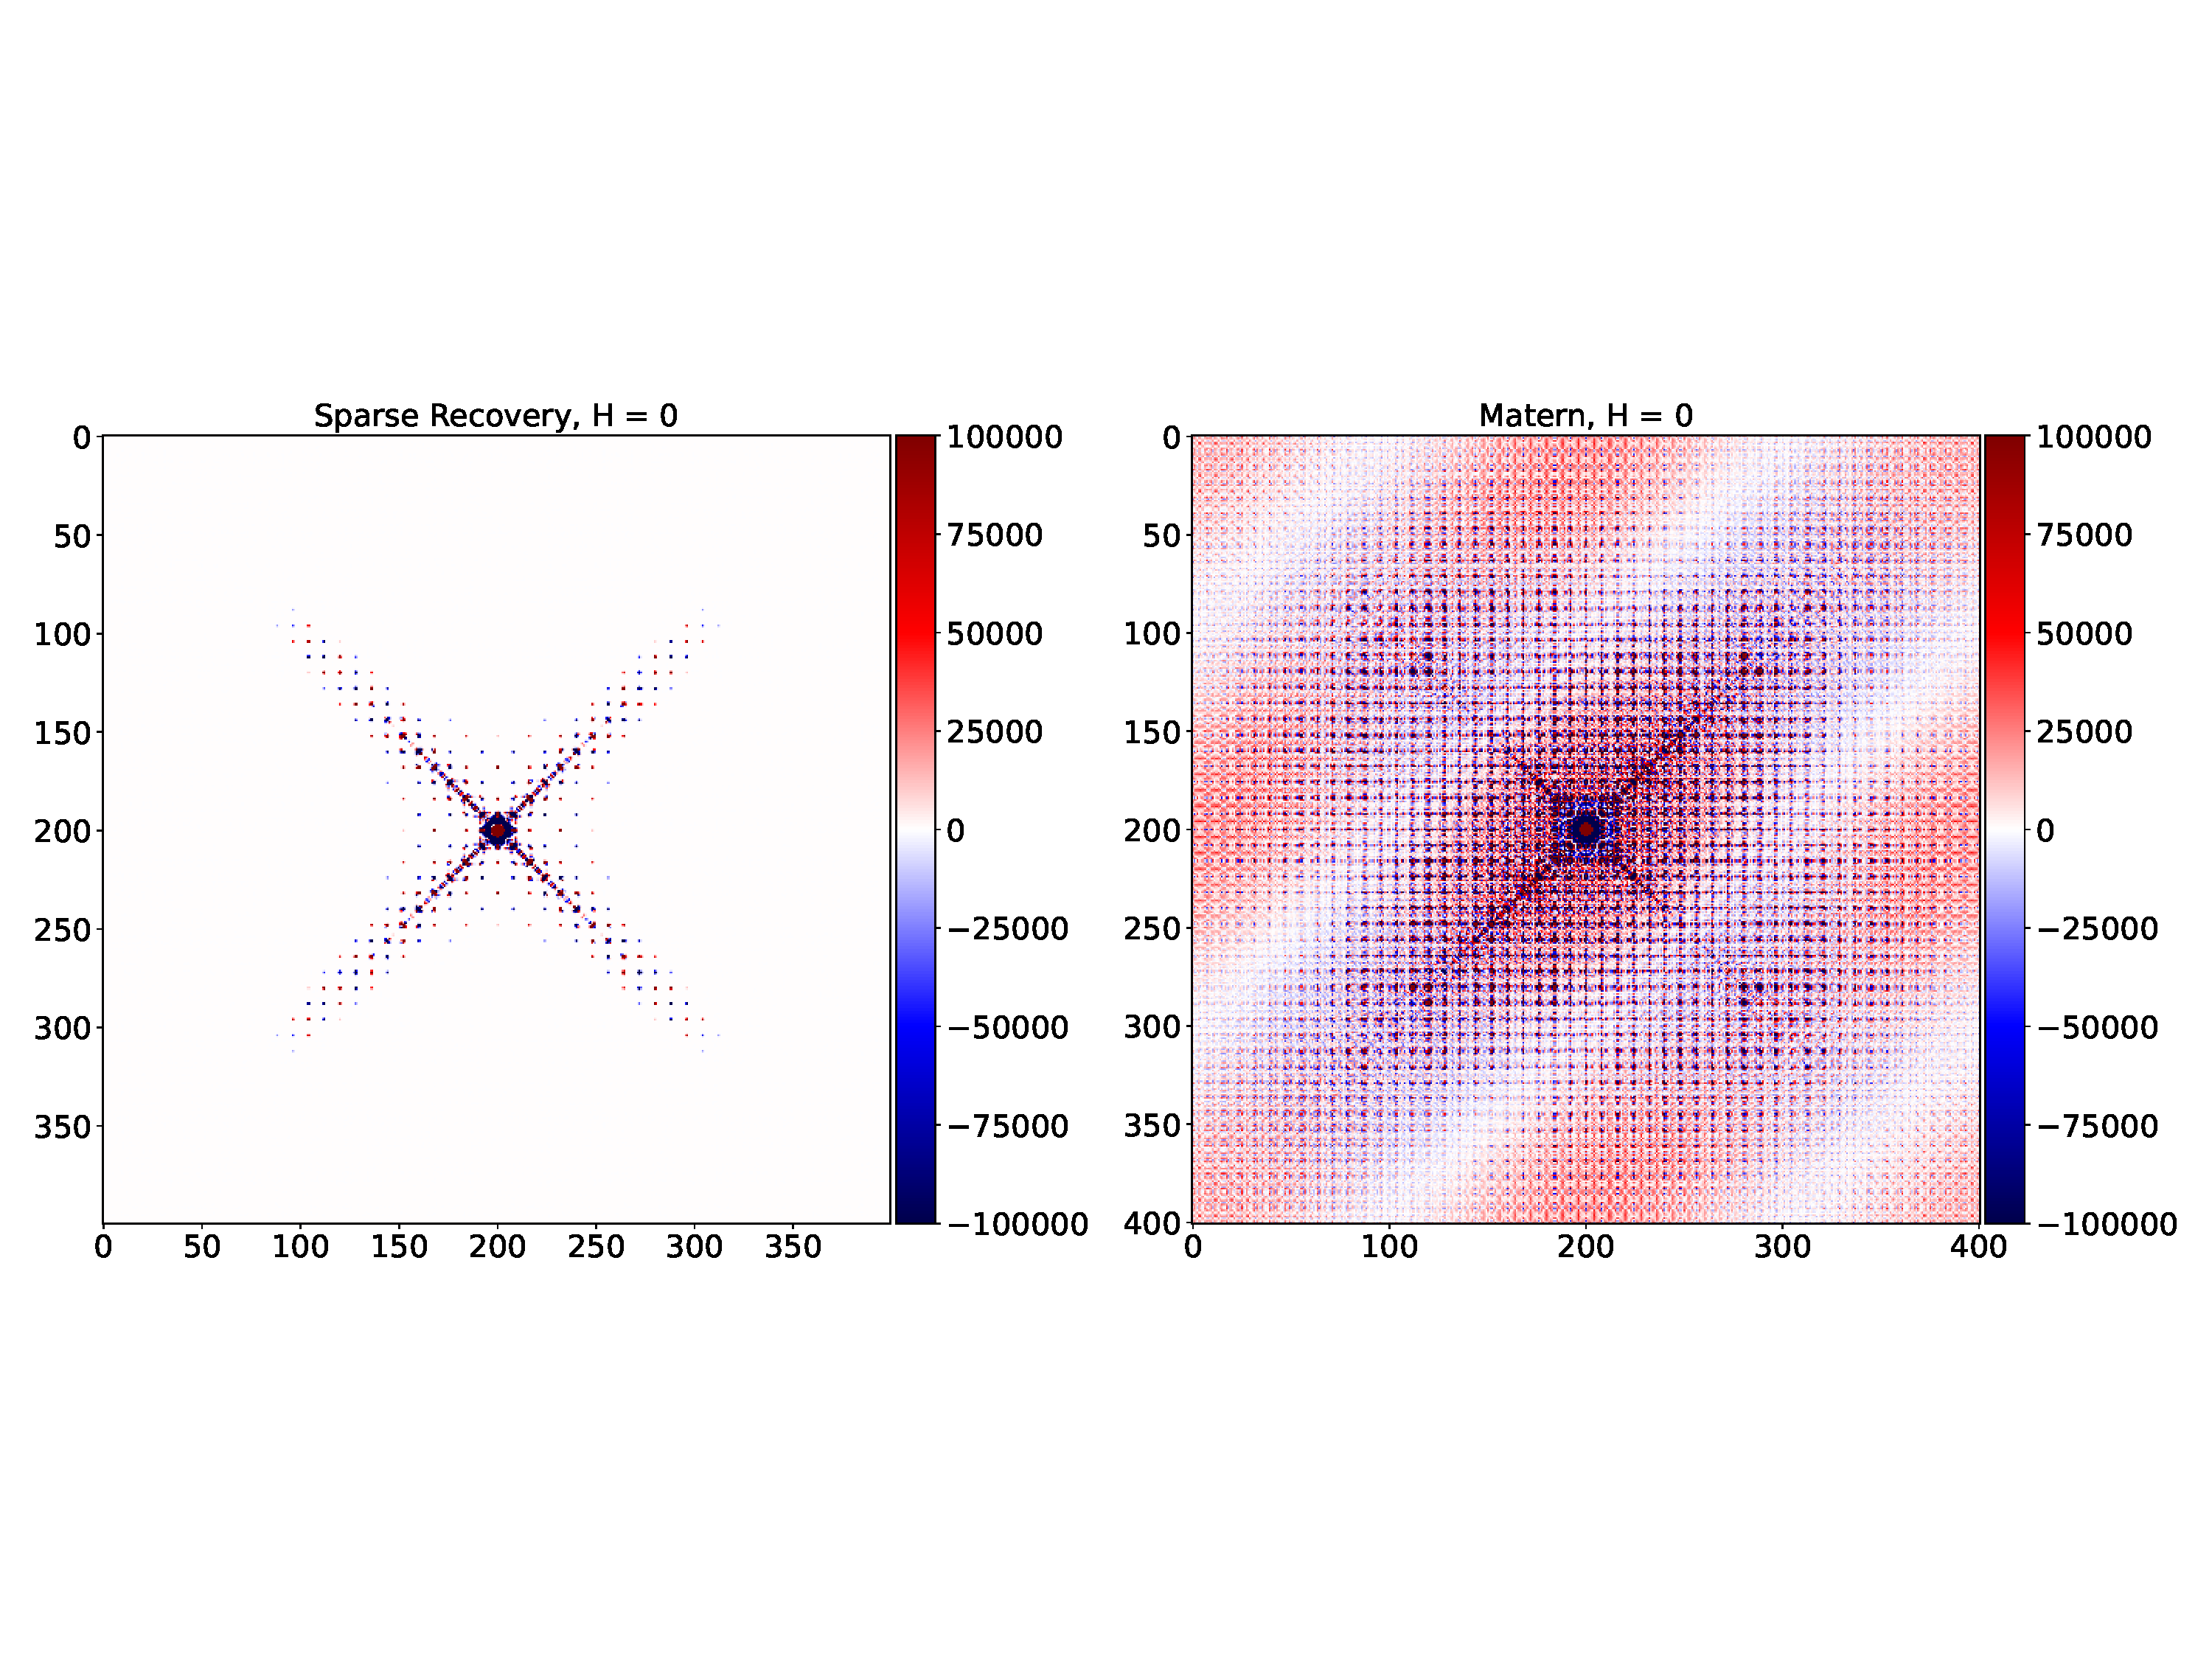
\includegraphics[width=\textwidth, trim=0in 4in 0in 4in 0in]{Figures/MaternVsSparse.pdf}
\caption{\label{fig:VO2} Left panel shows the sparse recovery, right panel shows ordinary punch and fill}
\end{figure}

Mathematically relevant to the study of the 3D-$\Delta$PDF is the notion that the
solution to the problem is inherently sparse, i.e. the PDF is essentially zero except
for some discrete features encoding pairwise interatomic vector probabilities
representing disorder in the crystal structure. Earlier approaches to this problem
involved removal of Bragg peaks using a punch-and-fill algorithm (including some
novel innovations of our own such as the \texttt{LaplaceInterpolation.jl} package, \cite{RH2022}) however the sharp edges
sometimes caused by the data interpolation could cause relatively large unintentional
ripples, or noise, in the resulting pdf. In order to mitigate this noise, we propose
a compressed sensing approach to solve the mathematical optimization problem which is characterized by an l1
constraint minimization. The punch-and-fill algorithm can be formulated as a problem of identifying the sparsity of Discrete Fourier transform (DFT) when the signal is noisy. Consider the noisy signal
\begin{equation}
    \widetilde{z} = \widetilde{x} + \widetilde{e}\,,
\end{equation}
we are in particular interested in the case where signal has some missing values, which intends to model the punching removal. Suppose the missing indices are recorded in a set $\mathcal{M}$. For simplicity, we denote our observed signal as
\begin{equation}
    z:=\widetilde{z}_{[n]\backslash\mathcal{M}},
\end{equation}
which are the observed values in the noisy signal. Then the loss function to minimize turns into $.$. 

Here we use the important insight that $v$ is sparse for many cases of interest. This can be mathematically enforced by adding an  $l_1$ constraint. Thus the resulting optimization problem becomes
\begin{equation}\label{eqn:complexopt}
    v = \arg\min_{v\in\mathcal{F}}\left\|z - \left(IFT(v)\right)_{[n]\backslash\mathcal{M}}\right\|_2 \text{ s.t. }\|v\|_1 \leq d,
\end{equation}
where the parameter $d$ characterize the sparsity of $v$. Alternatively, we can impose the sparsity constraint by using Lagrange multiplier, note that the objective is convex. We solve the above $l_1$ optimization problem using the alternating direction method of multipliers (ADMM)  approach and Figure \ref{fig:VO2} compares the results from interpolation and the compressed sensing approach. The left panel of the figure shows
the pdf using the compressed sensing algorithm (state parameters tuned here) in
comparison with the pdf calculated using the punch and fill algorithm, observe the vastly improved reconstruction. The reduction
of the low-profile noise to zero is the key advantage of the l1 minimization -
effectively reducing the complex features of the result to an interpretable set of
discrete interatomic vector probabilities. 

\subsection{An ADMM algorithm} The mapping $\left(IFT(v)\right)_{[n]\backslash\mathcal{M}}$ is a linear one in $v$ in problem \eqref{eqn:complexopt}. Therefore, by using the Lagrange multiplier approach to enforce the constraint of \eqref{eqn:complexopt} and replacing the objective using the classical notation $Ax=b$ for the underlying underdetermined linear system, and squaring the objective, the problem \eqref{eqn:complexopt} can be rephrased as 
\begin{equation} \label{}
    \text { minimize }(1 / 2)\|A x-b\|_{2}^{2}+\lambda\|x\|_{1}.
\end{equation}
To solve this convex nonsmooth optimization problem we use the alternating direction method of multipliers (ADMM). 
To start, we use a new variable and a penalty to state the equivalent problem
\begin{equation}
    \min_{x, z}(1 / 2)\|A x-b\|_{2}^{2}+\lambda\|z\|_{1} + \frac{\rho}{2}\|x-z\|^2,\text{ s.t. }x - z = 0.
\end{equation}
Since $\frac{\rho}{2}\|x-z\|^2$ is zero under the constraint $x - z = 0$ the two problems are identical. Using now a new Lagrange term for the constraint, we obtain
\begin{equation}
    \min_{x,z}\max_{y} L_{\rho}(x,z,y) = (1 / 2)\|A x-b\|_{2}^{2}+\lambda\|z\|_{1} + \frac{\rho}{2}\|x-z\|^2 + y^{\top}(x-z).
\end{equation}
The ADMM algorithm alternatively seeks the best objective by updating one variable at a time. 
\begin{equation}
    \begin{aligned}
x^{k+1} &:=\left(A^{T} A+\rho I\right)^{-1}\left(A^{T} b+\rho z^{k}-y^{k}\right) \\
z^{k+1} &:=S_{\lambda / \rho}\left(x^{k+1}+y^{k} / \rho\right) \\
y^{k+1} &:=y^{k}+\rho\left(x^{k+1}-z^{k+1}\right)
\end{aligned}
\end{equation}
where we have introduced the soft thresholding operator
\begin{equation}
S_{a}(x) = \begin{cases}x-a & x > a \\ 0 & -a\leq x\leq a\\ x+a & x<-a\end{cases}   \text{ for }a>0
\end{equation}
For problems of the size we are interested in, the first step is by far the most expensive. Since $A$ has orthogonal rows, we could use for the example we presented Sherman Morrison to reduce the computation to solving linear systems with matrices of the size of the few missing entries.  
However, for the larger problems we want to pursue here, we need even faster methods which underpins our proposed research. 





\subsection{Proposed Research} \label{ss:proposed}
Since our datasets can comprise over 100M pixels, the sparse recovery algorithm must be computationally efficient to be useful. The ADMM approach gives sparse and realistic 3D-$\Delta$PDF, but (a) we need to solve systems with the matrix $\left(A^{T} A+\rho I\right)$ faster and (b) we need even faster convergence if possible.  

For (a), we will explore iterative methods, which only require the action of matrices on vectors and do not store the entire matrix, to solve the linear system $\left(A^{T} A+\rho I\right) x = \left(A^{T}  b+\rho z^{k}-y^{k}\right) $. Matrix vector products with $A$ and its transpose can be implemented quasilinearily since it abstracts the Fourier transform and its inverse with truncation or zero padding. Therefore one way to go is to 
We propose to explore the use of conjugate gradient (CG) to solve the linear system. Initial results seem to indicate that the method works very well even not preconditioned, we will explore this further and pursue an analysis of this phenomenon to obtain a robust methods.  For (b) we will develop second order methods -- such as interior point algorithms --  which will result in much faster convergence as compared to the current ADMM approach. Note that the ADMM approach takes about a week to get reasonable reconstructions, whereas the Laplace interpolation approach takes only a few hours to solve the same problem, albeit with more noise as we indicated. The key for efficient interior point algorithms is the efficient resolution of the resulting Newton system;  this approximately requires solving a problem with matrix $AA^T+D$ where $D$ is now a matrix of penalty parameters which thus has vastly wider range compared to $\rho I$ and thus is more challenging to precondition. We will investigate effective preconditioners for this approach by means of an approximate active set approach followed by an analytical approximation on the inverse on that set. This will require us to develop efficient matrix free methods that exploit the structure of the problem.

%\new{\textbf{Summary}}

%\new{\textbf{What we have done:} \begin{itemize}
%    \item Laplace Interpolation package for full 3D Volume dataset (this has been incorporated into the workflow).
%    \item Compressed sensing approach using ADMM for the full 3D Volume dataset (Vo2 data)
%\end{itemize}}

%\new{\textbf{What we plan to do:}  \begin{itemize}
%    \item Develop/Incorporate second order methods for the compressed sensing to accelerate the convergence of the optimization.
%    \item Accelerate the linear algebra components involved in the compressed sensing approach (Matrix-free methods, iterative methods, parallelism to take advantage of the dense structure etc.)
%\end{itemize}}


% The conjugate structure of DFT makes the optimization in complex field difficult. However, this can be reformulated as a LASSO in real field. Multiple first order and second order methods can be applied to solve the problem Besides, the orthogonal structure of inverse Discrete Fourier transform (IDFT) allows us to greatly reduced the storage. Also the operations of computing Newton direction is linear in problem size. Thus, our method is practical and scalable. 
% While such datasets can comprise over 100M pixels, the
% sparse recovery algorithm must be computationally efficient to be useful. This is the
% case for the Vo2 dataset pictured in the figure. The left panel of the figure shows
% the pdf using the compressed sensing algorithm (state parameters tuned here) in
% comparison with the pdf calculated using the punch and fill algorithm. The reduction
% of the low-profile noise to zero is the key advantage of the l1 minimization -
% effectively reducing the complex features of the result to an interpretable set of
% discrete interatomic vector probabilities. 
% This work was computed in collaboration with Wei Kuang, University of Chicago. 

% Compressed sensing is done by many people but it is not clear that they do it with
% enhanced computational speed. Nobody else has a second order method, etc. etc.
% Descriptors that explain what we are doing differently.
